\chapter{The FNAL Recycler Ring}
\label{sec:ch3}

\section{\label{sec:intro31}Introduction}
The Fermilab Recycler Ring (RR) is one of the circular accelerators located in the Fermilab Accelerator Complex. It was originally designed to store and accumulate antiprotons that remained from a Tevatron event \cite{rr0}. The recycling of antiprotons was deemed ineffective and was never operationally implemented \cite{rrnagaitsev}. Since 2011, the RR has been repurposed to act as a pre-injector to the Main Injector (MI) by storing and accumulating protons \cite{rr1}. It is worth pointing out, that the MI and the RR share the same tunnel, which has a circumference of 3.319 km (2.062 mi). The work done for this thesis focuses on the Recycler Ring. The following chapter starts by giving a general description for the operation and physics of the Recycler Ring. The next sections introduce and motivate the compensation of third order resonances for high intensity operation.  

The MI/RR complex is fed protons by the Proton Source, which by itself consists of the Pre-Accelerator, the Linear Accelerator (Linac), and the Booster. The Pre-Accelerator systems provide $H^-$ ions to the Linac, where they are accelerated to an energy of 400 MeV. After this, the beam is injected into the Booster Ring. The Booster is a rapid-cycling synchrotron operating at a 15 Hz repetition rate. During this injection process, the $H^-$ beam passes through a carbon stripping foil, and it incorporates to the circulating proton beam. The Booster ramps the energy up from 400 MeV to 8 GeV. This 8 GeV proton beam can either go to the Booster Neutrino Experiments or get injected into the Recycler Ring. Once in RR the beam has two possible destinations: 1) high energy neutrino experiments through MI or 2) Muon Campus. For the latter, proton beam gets rebunched from 53 MHz to 2.5 MHz and transported to Muon Campus. For high energy neutrino experiments, the proton beam gets slip-stacked, hence doubling the intensity that gets injected into Main Injector. Once in MI, the beam is accelerated to 120 GeV and sent to the NuMI (Neutrinos at the Main Injector) beam facility \cite{rr1, rrnagaitsev, numi1}. A description of the current accelerator complex is shown in figure \ref{fig:fnal}, including the experimental beamlines which feed neutrino, muon and fixed target experiments.

\begin{figure}[H]
   \centering
   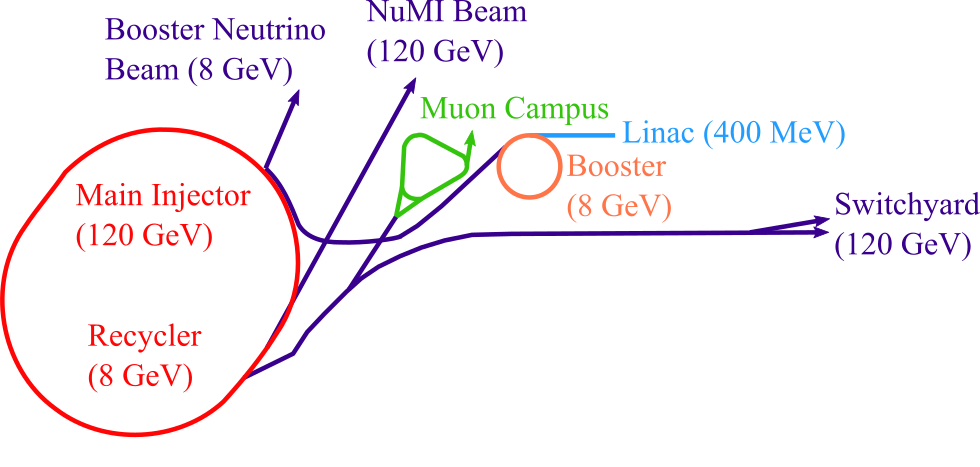
\includegraphics[width=\columnwidth]{chapter3/complex_noTev.png}
   \caption{Current operational layout of the Fermilab Accelerator Complex as of 2024. Original plot provided by R. Ainsworth, first published on Ref. \cite{rr1}, but modified for this document.}
   \label{fig:fnal}
\end{figure}

The Proton Improvement Plan II (PIP-II) is the first step in establishing the Fermilab Accelerator Complex as a multi-MW proton facility \cite{pipII1}. The near-future objective is to deliver a 1.2 MW proton beam to the Deep Underground Neutrino Experiment (DUNE) through the Long-Baseline Neutrino Facility (LBNF) \cite{dune}, still in construction. In order to meet this goal, several upgrades are being planned in the accelerator complex, including a new 800 MeV superconducting linear accelerator. The future plan for the layout of the Fermilab Accelerator Complex is shown in Fig. \ref{fig:fnalpip2}. With minimal upgrades to the Main Injector and Recycler Ring, but with a substantial overhaul of the Booster Ring, this will allow for a 50\% increase in particles per pulse intensity. Table \ref{tab:rrparams} also specifies some upgrades that will happen for the PIP-II era. Some examples include an increase of the particle per bunch intensity, a shortening of the Main Injector acceleration ramp and an increase in the Booster ramping rate. As the Recycler Ring starts to deal with higher intensities from the PIP-II upgrade, it is important to mitigate the effects of space charge as discussed in Secs. \ref{sec:resonances} and \ref{sec:sc1}. Particles along the bunch will experience space charge forces leading to detuning in their betatron frequencies. Given the incoherent nature of this process, this leads to the beam having a larger tune spread in the tune diagram and having particles operate on top of resonances.

\begin{figure}[H]
   \centering
   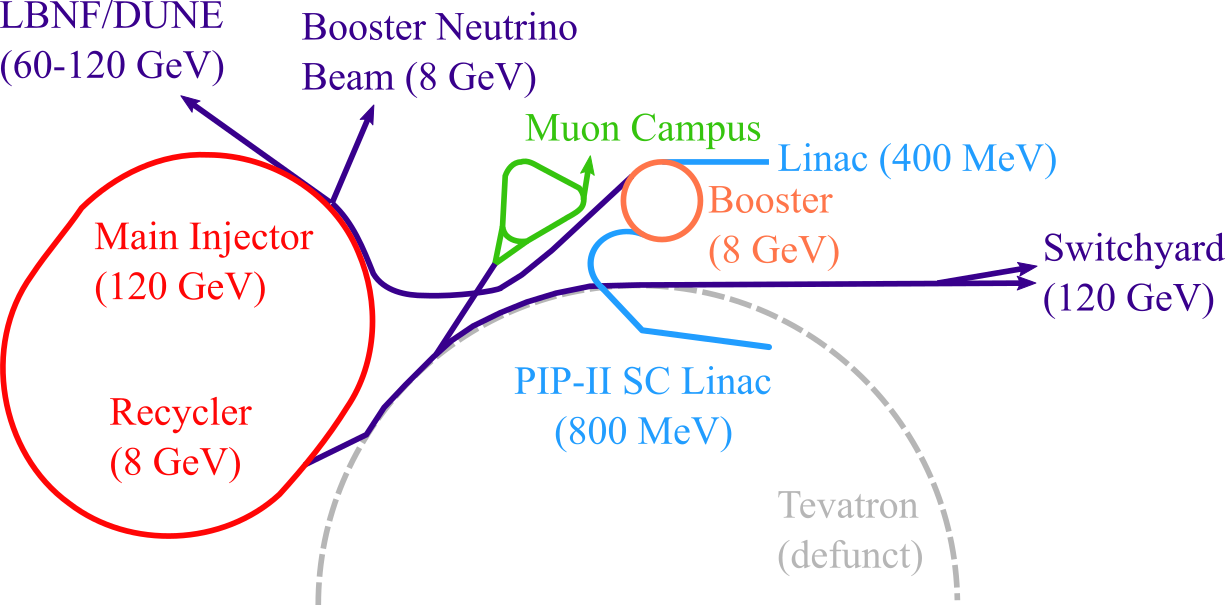
\includegraphics[width=\columnwidth]{chapter3/complexPIPII.png}
   \caption{Future layout of the Fermilab Accelerator Complex for the Proton Improvement Plan II (PIP-II). Original plot provided by R. Ainsworth, first published on Ref. \cite{rr1}, but modified for this document.}
   \label{fig:fnalpip2}
\end{figure}

\section{\label{sec:rrgen}General Description}

The RR is a permanent magnet storage ring operating at a fixed momentum of 8.835 GeV/c equivalent to an energy of 8 GeV. The basic cell structures of this machine are FODO (Focusing Quadrupole - Drift - Defocusing Quadrupole - Drift) cells. During its conception, the need for a quick and non-expensive design spurred the idea of combining quadrupole and dipole magnets into one combined function magnet. These combined function magnets can be seen in Fig. \ref{fig:rrtunnel} as the green covered magnets on the top ring---the Recycler Ring. In order to further reduce costs during its construction, these magnets were chosen to be permanent magnets made out of a strontium ferrite \cite{rr0}. Some advantages of having permanent magnets is that there is no need for power supplies, cooling systems or power distribution cables. Consequently, these type of magnets are very stable against time and temperature. Nevertheless, the magnetic field of such magnets does degrade over time. Reference \cite{rr1} shows how the fields in RR-type magnets can degrade around 1\% after 20 years. Ultimately, this slightly changes the nominal energy in the machine. 

\begin{figure}[H]
   \centering
   \includegraphics[width=\columnwidth]{chapter3/tunnel.jpg}
   \caption{Picture of the Main Injector (blue and red magnets in the bottom) and the Recycler Ring (green magnets up top) tunnel.}
   \label{fig:rrtunnel}
\end{figure}

Figure \ref{fig:rrtunnel} reminds the reader that the Main Injector and the Recycler Ring share the same tunnel. This tunnel is divided into six sections with labels: 100, 200, 300, 400, 500 and 600. Injection from the Booster Ring into the Recycler takes place just after the beginning of section 100. Specifically, this happens at a Lambertson magnet labelled as LAM102. This is just an example of how every element in the RR or MI will be labelled according to their position in one of these sections. Figure \ref{fig:rrschematic} shows a schematic of the Recycler Ring section with some labels for important subsystems inside them. In particular, it shows the location close to 232 where beam is transferred from the Recycler Ring to the Main Injector. Figure \ref{fig:rrschematic} also presents the location in section 500 where beam is transferred from RR to the Muon Campus, as well as the location after 401 where beam is dumped towards the abort line \cite{rr1,fermi_rookie}.

An important subsystem as highlighted in Fig. \ref{fig:rrschematic} is the tune trombone. The RR has two of them, one located in sections 601-609 and another one in 301-309. A tune trombone or phase trombone is a linear insert composed of quadrupoles used to introduce local phase advances. These quadrupoles are powered in such a way that they add a controlled phase advance, while leaving the Twiss parameters unchanged at the end of the insert and matched to the start of the trombone \cite{trombone,rr0}. Ultimately, these subsystems introduce local tune changes that allow to control both tunes in a range of $\pm 0.5$, i.e., $\Delta Q_u = \pm 0.5$. The Recycler Ring has accelerator applications that allow to control these tune trombones and set the tunes to some desired values. Furthermore, this application allows introducing tune ramps, continuous linear changes in the tunes. This feature is crucial for building dynamic loss maps---an important tool to probe resonance lines as will be described in Sec. \ref{sec:lossmaps}.    

\begin{figure}[H]
   \centering
   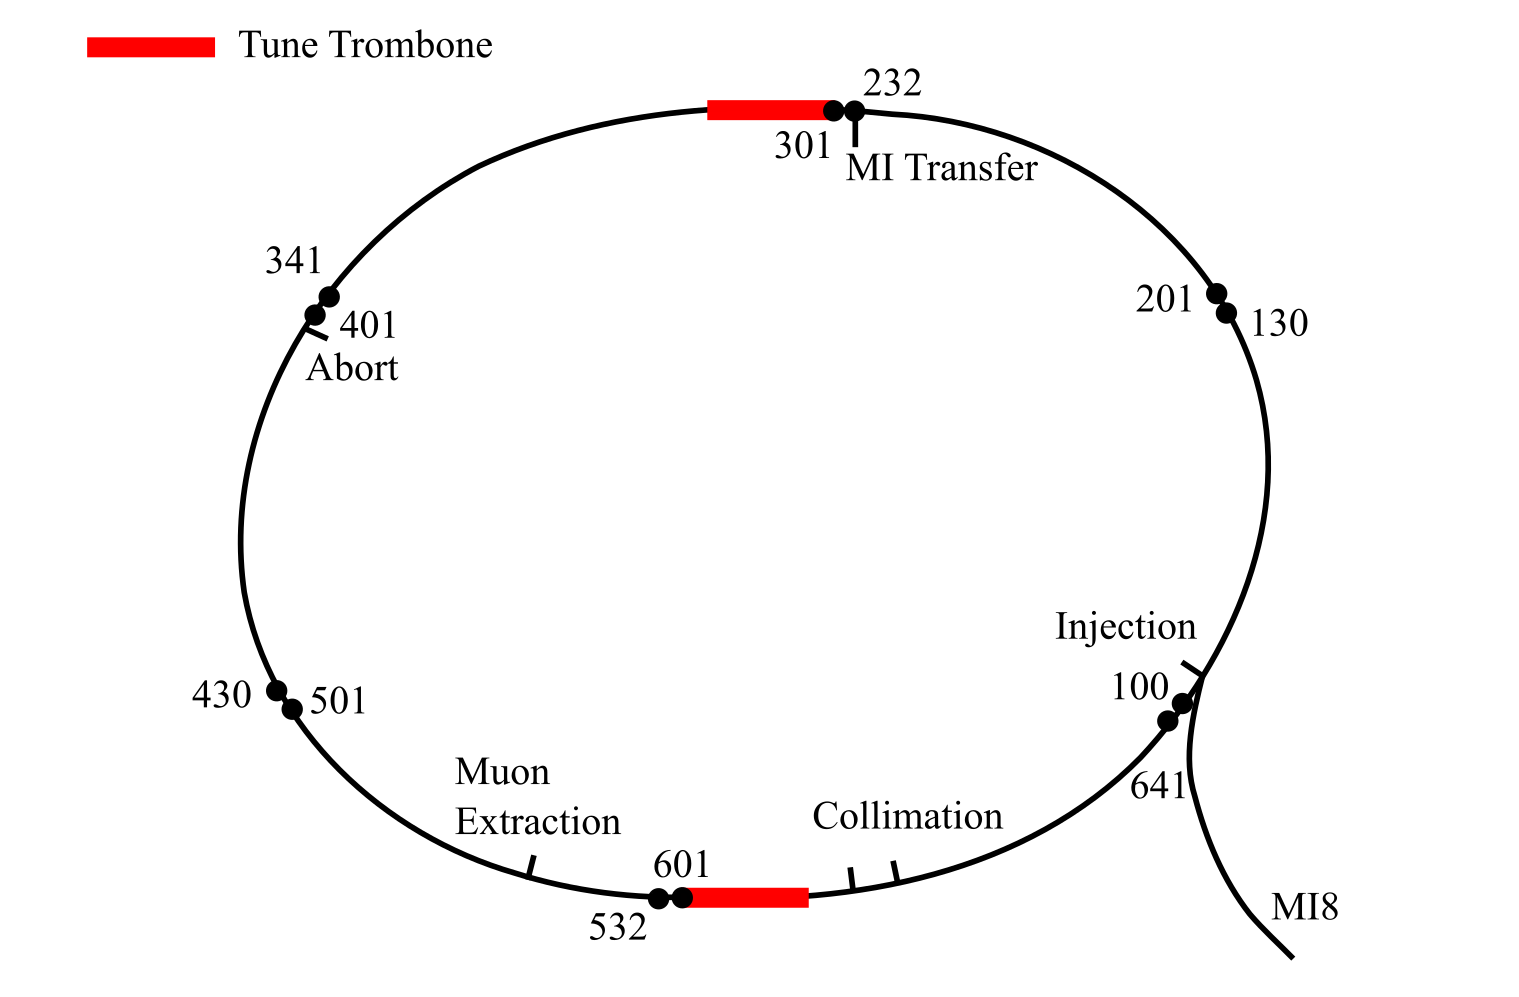
\includegraphics[width=\columnwidth]{chapter3/RRschematic.png}
   \caption{Schematic layout of the Recycler Ring and its corresponding sections. Original plot provided by R. Ainsworth, first published on Ref. \cite{rr1}.}
   \label{fig:rrschematic}
\end{figure}

The Recycler Ring has 104 FODO cells distributed into 3 main groups around its 3319.4-meter circumference \cite{rr0}. The first group of cells are composed of two permanent magnet quadrupoles arranged in such a way that each cell has a phase advance of 90$^{\circ}$. There are 18 cells of this first group throughout the Recycler. The second group is defined by a cell with two combined function magnets in order to bend and focus the beam at the same time. This type of cell also has a phase advance of 90$^{\circ}$, with 54 cells of this type in the RR. Ultimately, the configuration of these cells will dictate the Twiss parameters around the ring. Figure \ref{fig:rrbetas} shows the beta functions $\beta_u(s)$ around the Recycler Ring tuned to some particular set of tunes. Some horizontal BPMs are marked in the upper horizontal axis as reference to note the corresponding section in the tunnel.    

Before describing the third group, it is worth clarifying to the reader that the transverse motion inside any circular accelerator is dictated by:
\begin{equation}
   \label{eq:utotal}
   u(s) = u_{\beta}(s) + D_u(s) \delta,
\end{equation}
where $u$ is either the $x$ or $y$ plane, $u_{\beta}(s)$ is the betatron motion as described by Eq. \ref{eq:betatron}, $D_u(s)$ is known as the dispersion function and $\delta=\Delta p/p_0$ is the fractional momentum deviation of an individual particle with respect to reference longitudinal momentum $p_0$. In Ch. \ref{sec:ch2}, specifically in Sec. \ref{sec:lie}, an assumption was made that the transverse coordinates were not going to be influenced by any longitudinal property, focusing on on-momentum particles, i.e., $\delta =0$. Nevertheless, for this section it is relevant to introduce the dispersion function $D_u(s)$ in order to describe the Recycler Ring in all its glory and detail. The dispersion function is dictated by the distribution of quadrupole and dipole component throughout the ring \cite{sylee}. Even so, the scope of this work regarding resonance compensation will not take into account any longitudinal-transverse coupling.   

With all this said, the third group of cells is composed of special dispersion suppressor cells, $D_x(s)=0$ for these regions. Each one having two combined function magnets and globally having a betatron phase advance of again 90$^{\circ}$. This type of cells will allow having dispersion-free regions which are necessary for injection, extraction and other special subsystems in the Recycler. There are 32 cells of this type. Figure \ref{fig:rrdisps} shows the dispersion functions for the Recycler Ring. The horizontal dispersion function $D_x(s)$ has regions of close-to-zero values thanks to this third type of FODO cells. The vertical dispersion is effectively negligible, i.e., $D_y(s)\approx 0$.

\begin{figure}[H]
   \centering
   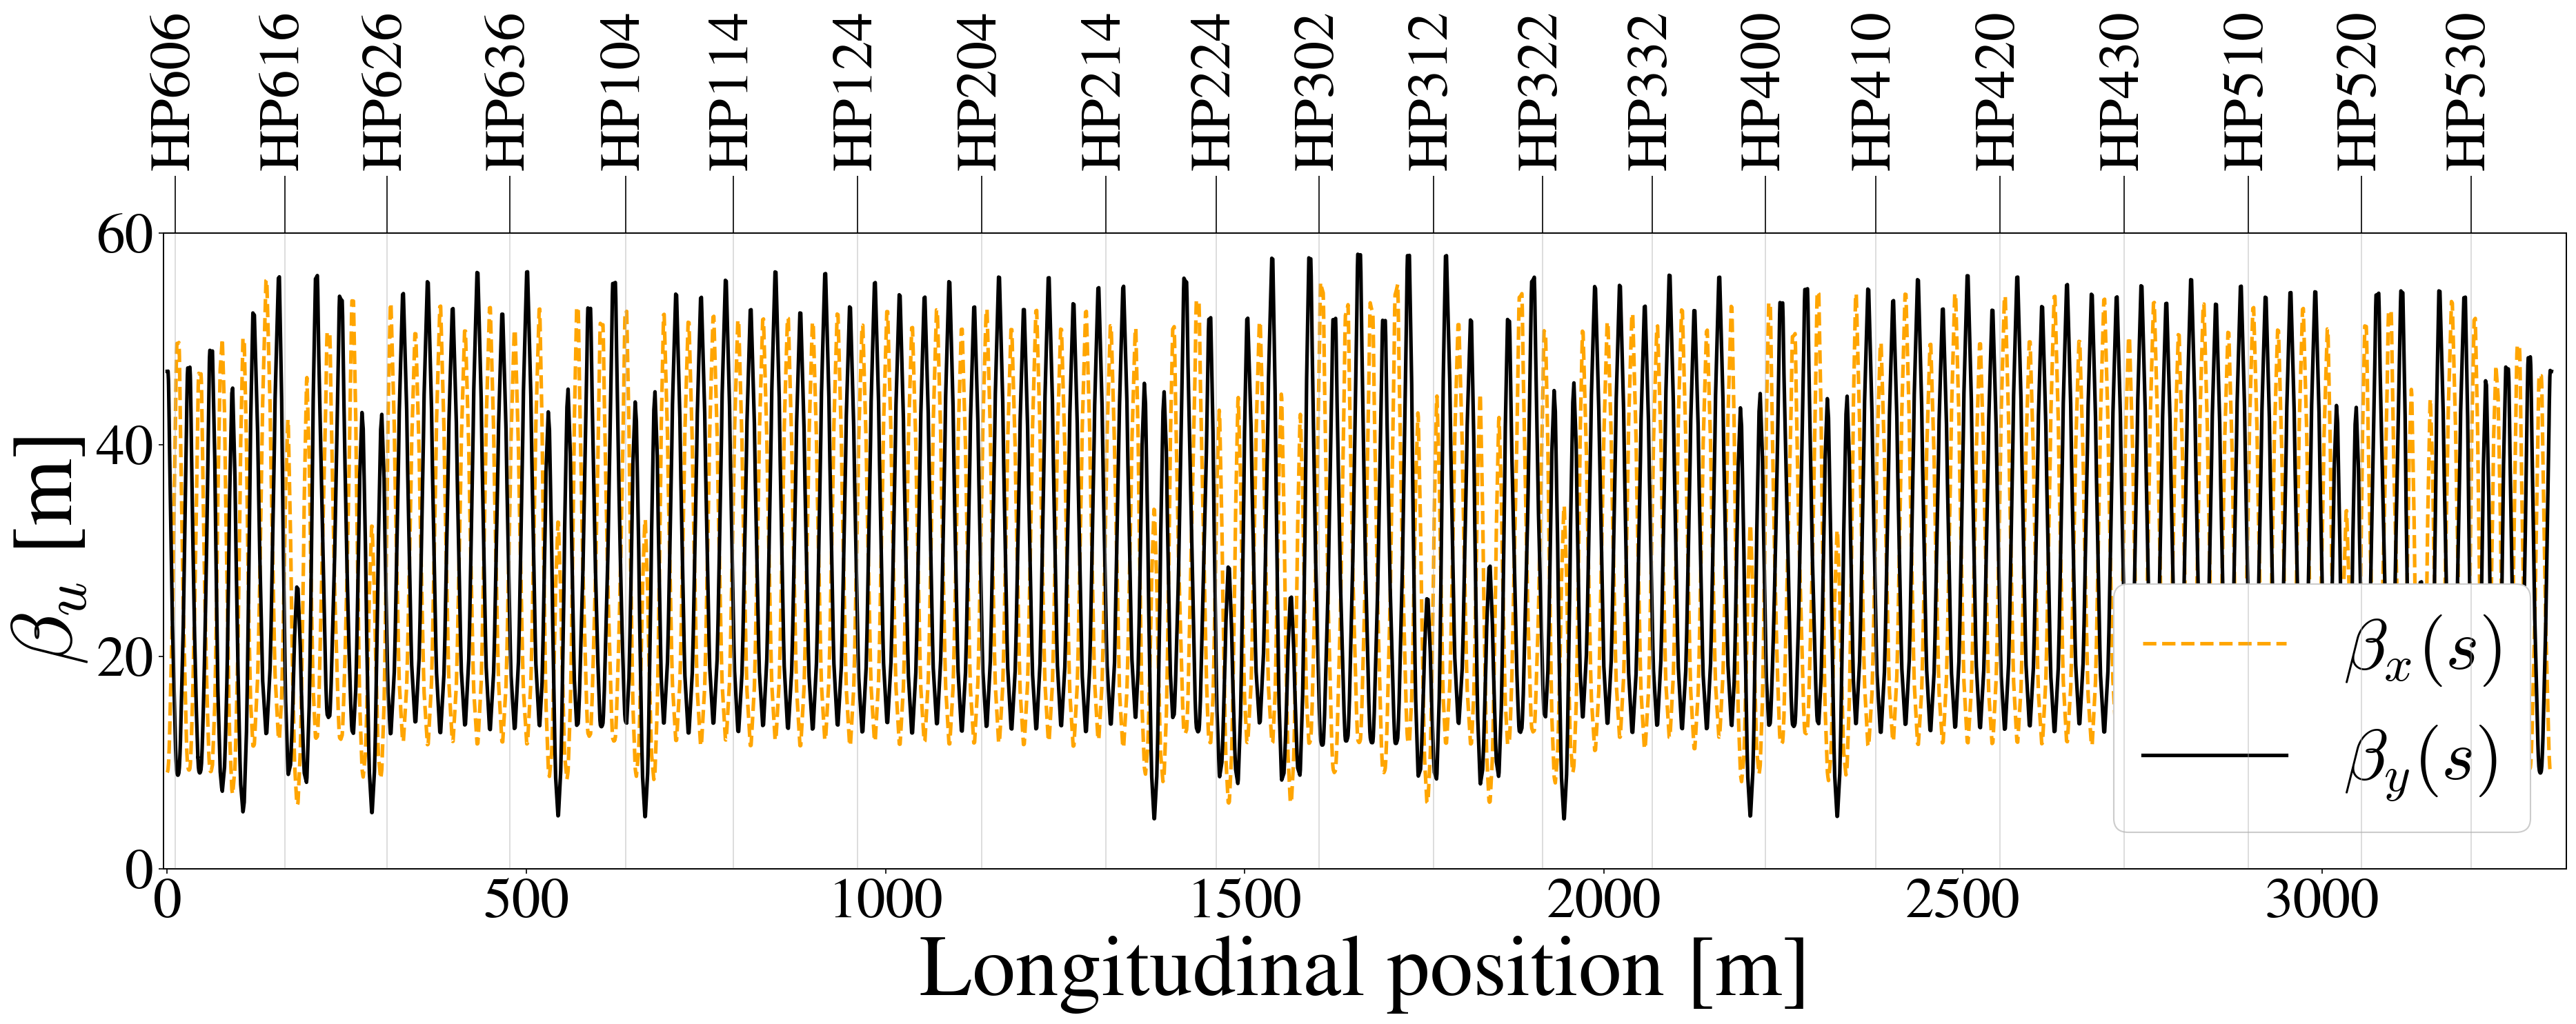
\includegraphics[width=\columnwidth]{chapter3/betas.png}
   \caption{Beta functions for the Recycler Ring lattice tuned to $Q_x=25.44$ and $Q_y=24.39$. Lattice functions calculated from lattice file using SYNERGIA.}
   \label{fig:rrbetas}
\end{figure}

\begin{figure}[H]
   \centering
   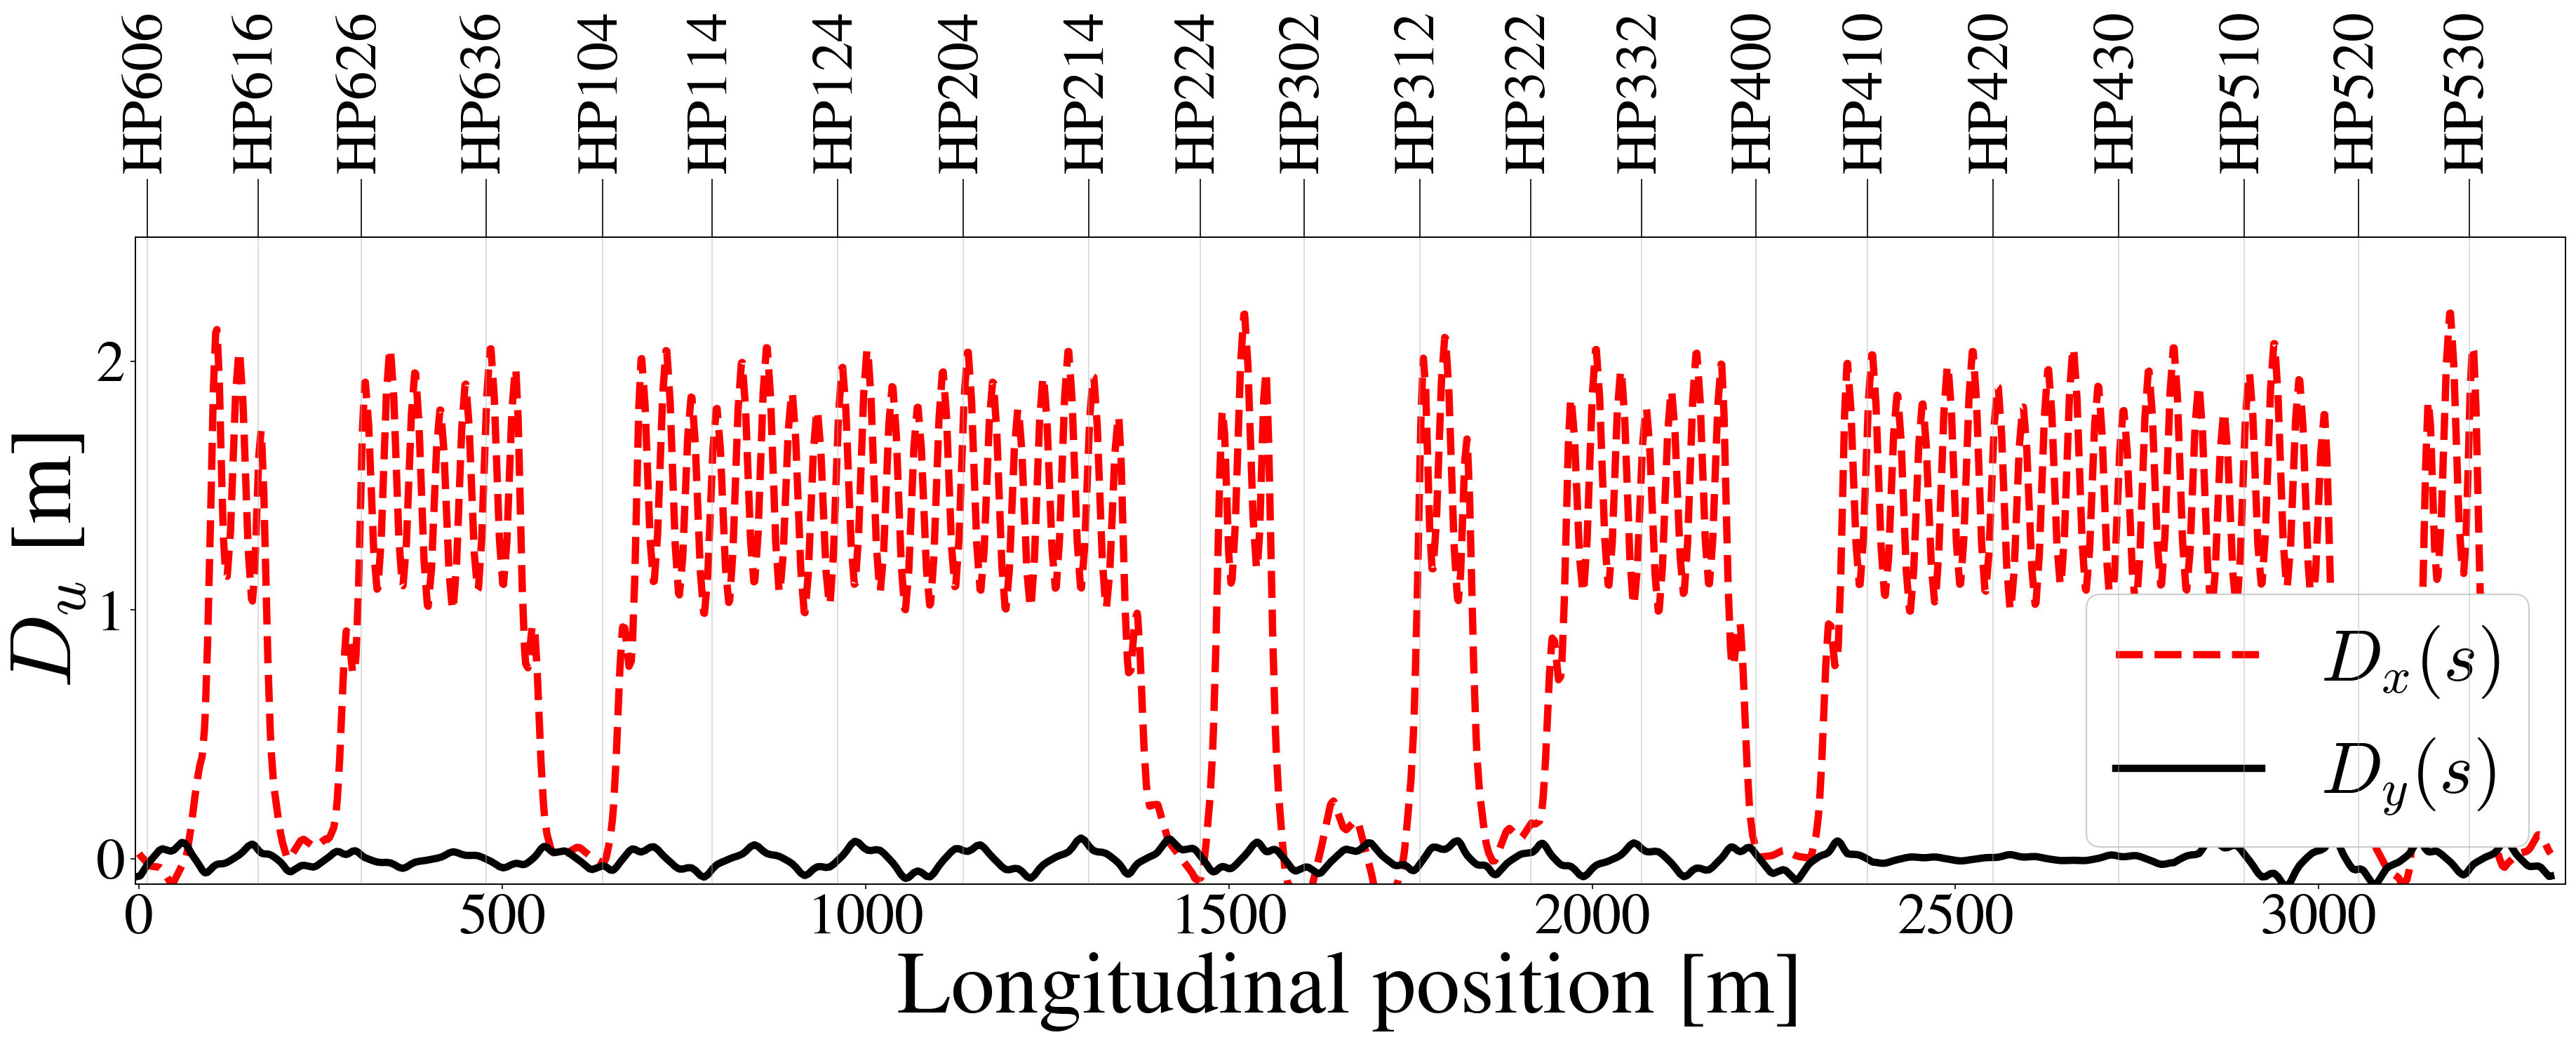
\includegraphics[width=\columnwidth]{chapter3/disps.png}
   \caption{Dispersion functions for the Recycler Ring lattice tuned to $Q_x=25.44$ and $Q_y=24.39$. Lattice functions calculated from lattice file using SYNERGIA.}
   \label{fig:rrdisps}
\end{figure}

The ultimate role of the Recycler Ring is to smooth the way for high-intensity proton beam injection into the Main Injector. In particular, for the high-intensity beam that gets delivered to the neutrino experiments, the Recycler performs a beam manipulation known as slip-stacking. Although this longitudinal manipulation is out of the main scope of this thesis, it is relevant to briefly explain this procedure since this is the Recycler Ring's main feature. Slip-stacking is the process through which a pair of bunches are manipulated in longitudinal phase space in order to merge them into one higher-intensity bunch \cite{fermi_rookie}. In particular, the RR utilizes two RF stations to decelerate and accelerate trains of bunches. The Recycler can fit 7 Booster Rings, hence 6+6 beam batches are injected and slip-stacked, while 1 batch space is left as a gap for the kickers to fire. Each batch is composed of 81 bunches in accordance to the harmonic number of the Recycler. A more detailed explanation of the Recycler Ring's slip-stacking procedure can be found in Refs. \cite{rr1,rr2,fermi_rookie}. Ultimately, this slip-stacking process is relevant because it doubles the particles per bunch intensity (ppb) which has important consequences for the transverse dynamics, as explained in Sec. \ref{sec:sc1}. Furthermore, Table \ref{tab:rrparams} summarizes some important parameters for the RR slip-stacking and for the general operation of neutrino-bound beam.     

\begin{table}[H]
   \centering
   \caption{Typical Recycler Ring properties for beam sent to NuMI, with some PIP-II nominal parameters.}
   \label{tab:rrparams}
   \begin{tabular}{@{}ccc@{}}
   \toprule
   \textbf{Parameter}          & \textbf{Value}                             & \textbf{Unit} \\ \midrule
   Circumference               & 3319.4                                     & m             \\
   Momentum                    & 8.835                                      & GeV/c         \\
   Revolution Period           & 11.1                                       & $\mu$s        \\
   Revolution Frequency        & 90.1                                       & kHz        \\
   RF Frequency                & 52.8                                       & MHz           \\
   RF Voltage                  & 80                                         & kV            \\
   Harmonic Number             & 588                                        &               \\
   Synchrotron Tune            & 0.0028                                     &               \\
   Slip Factor                 & -8.6 $\times$ 10$^{-3}$                    &               \\
   Superperiodicity            & 2                                          &               \\
   Horizontal Tune             & 25.43                                      &               \\
   Vertical Tune               & 24.445                                     &               \\
   Horizontal Chromaticity     & -6                                         &               \\
   Vertical Chromaticity       & -7                                         &               \\
   95\% Normalized Emittance   & 15                                         & $\pi$ mm mrad \\
   95\% Longitudinal Emittance & 0.08                                       & eV s          \\
   Intensity                   & $5\times10^{10}$                           & ppb           \\
                               & $8\times10^{10}$ (PIP-II)                  & ppb           \\
   MI Ramp Time                & 1.2                                        & s             \\
                               & 1.133                                      & s             \\
                               & 1.067                                      & s             \\
   Booster Frequency           & 15                                         & Hz            \\
                               & 20 (PIP-II)                                & Hz            \\ \bottomrule
   \end{tabular}
   \end{table}

\section{Tune Diagram and Resonances}

Table \ref{tab:rrparams} specifies nominal horizontal and vertical tunes for the operation of the Recycler Ring. While this pair of tunes can be switched around during operation in order to reduce losses, they will always stay clear of the surrounding transverse betatron resonances, as introduced in Sec. \ref{sec:resonances}. The resonance lines that are relevant to the Recycler Ring operation are plotted in Fig. \ref{fig:rrtd}, with their corresponding order in the multipole expansion. Specifically, this study looks at normal sextupole lines $3 Q_x=76$ and $Q_x+2Q_y=74$, plus skew sextupole lines $3 Q_y=73$ and $2 Q_x+Q_y=75$.

\begin{figure}[H]
   \centering
   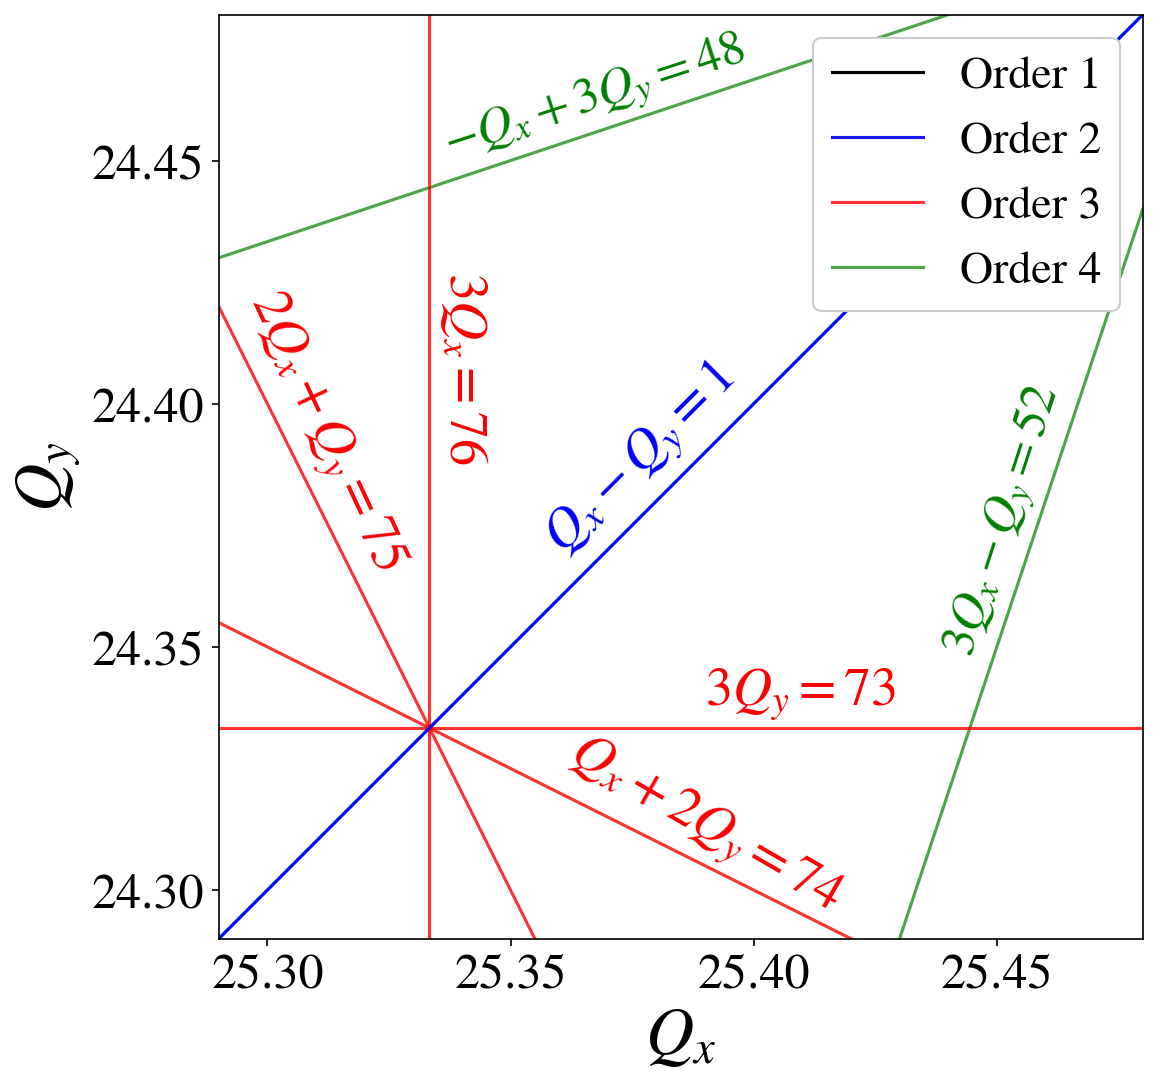
\includegraphics[width=\columnwidth]{chapter3/rrtd.png}
   \caption{Portion of the tune diagram enclosing the operational tunes of the Recycler Ring.}
   \label{fig:rrtd}
\end{figure}

Starting from the lowest order resonance line, Fig. \ref{fig:rrtd} shows the second-order linear coupling line $Q_x-Q_y = 1$. This resonance line comes from skew-quadrupole component accumulated all around the ring. While operating on top of this resonance line won't lead to chaotic motion, the dynamics are characterized by action-exchange between the betatron modes \cite{sylee}. This exchange can cause emittance growth, eventually leading up to beam loss. Due to this fact, the Recycler Ring has two families of skew quadrupoles in order to correct this resonance line. Consequently, operating close to this resonance line is feasible with this correction.

The third order resonance lines are the main focus of this thesis. They are driven by normal and skew sextupole component distributed all around the ring. In particular, it is known that the combined function magnets are the main drivers of these resonance lines. Even though these magnets were designed to be quadrupole and dipole only, they can still have sextupole component from construction errors. Nevertheless, since they are permanent magnets little can be done about the magnets themselves. As a result of this, the following work explores a compensation technique aimed towards bringing down the lattice RDTs that drive these resonance lines. This involves the usage of additional compensation sextupoles, elements which will be described in Sec. \ref{sec:css}. Chapter \ref{sec:ch4} goes into a deep dive explaining this approach from a theoretical and experimental point of view. 

Finally, there are also fourth order resonance lines close to the nominal operation of the Recycler. These lines are driven by octupole components around the ring. In practice, $-Q_x+3Q_y = 48$ and $3Q_x-Q_y = 52$ are not particularly concerning to the operation of the RR. Their corresponding lattice RDTs are not large enough to consider them dangerous during the RR cycle, i.e., beam is stored for approximately 1 second. Nevertheless, these lines are interesting because fourth order resonance lines are susceptible to be amplified by the space charge potential through the SCRDTs, as described in Sec. \ref{sec:sc1}.    

\section{High Intensity and Tune Footprint}

In order to achieve the PIP-II beam power objective, the Recycler will be required to store and accumulate 50\% more beam than current operations \cite{pipII1}. As it was explained in Sec. \ref{sec:sc1}, larger beam intensities lead to larger space charge tune spread. Figure \ref{fig:rrtdhigh} shows how for typical operation to the neutrino experiments under future PIP-II specifications, there is a space charge tune spread of around 0.1 in both planes. At nominal tunes, it is clear that for high intensity operation the particles in the core of the beam will start to operate on top of third order resonances. One thing complicates this picture further, which is that particles will undergo synchrotron oscillations within the diamond shape region. This means that particles will go from the core of the beam to its outskirts, and its incoherent space charge tune shift will fluctuate accordingly. Therefore, particles will be crossing in and out of these third order resonances at a synchrotron period. Ultimately, Fig. \ref{fig:rrtdhigh} just tries to take a snapshot of the region of these excursions.  

\begin{figure}[H]
   \centering
   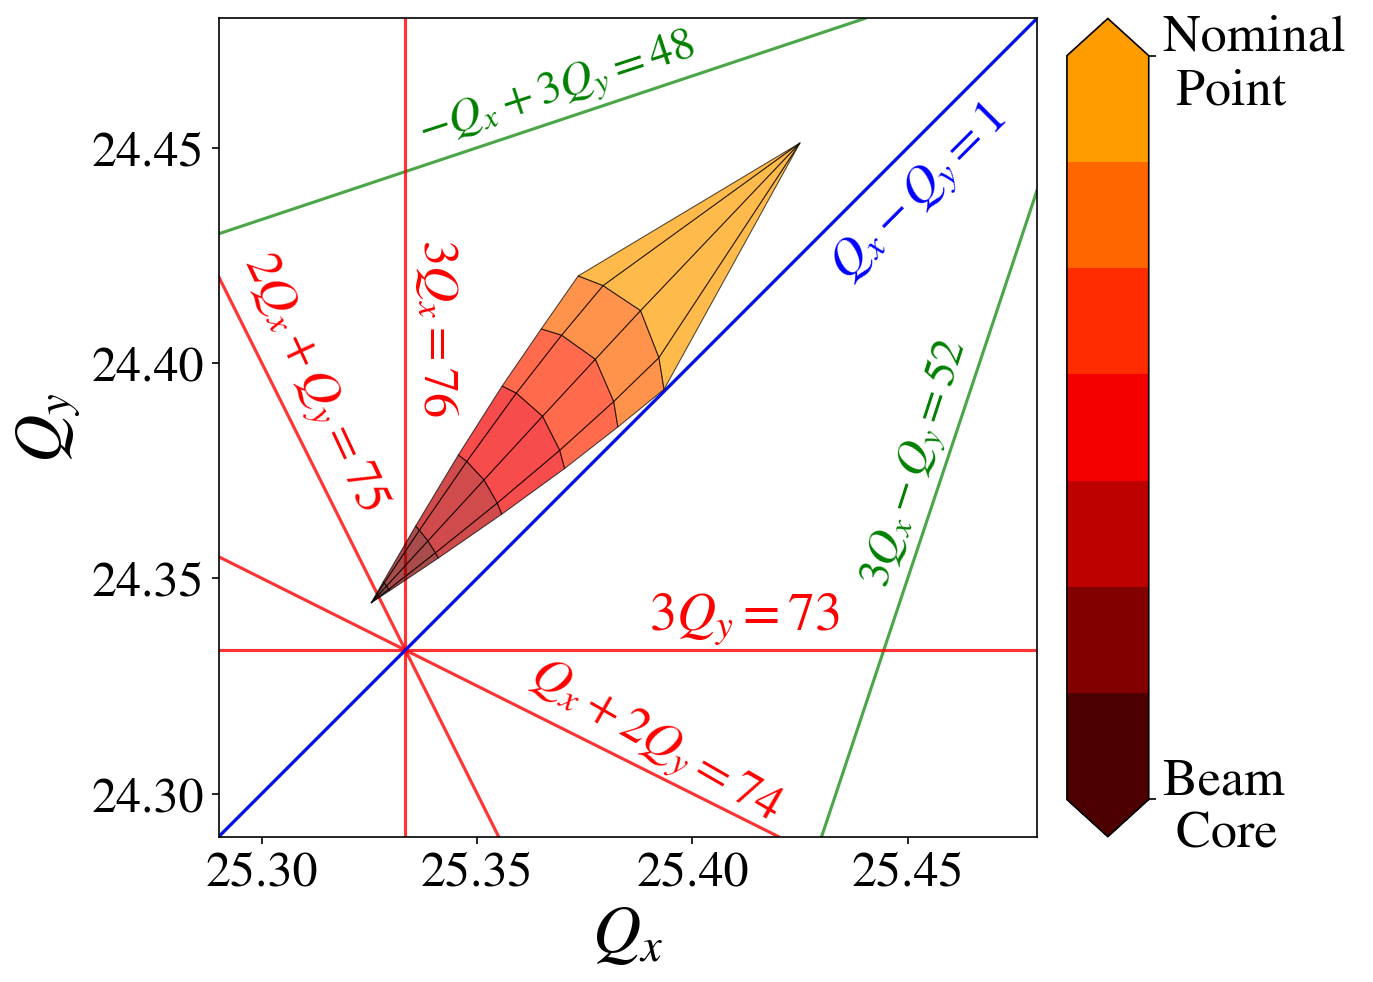
\includegraphics[width=\columnwidth]{chapter3/rrtdhigh.png}
   \caption{Approximate operational tune footprint at high intensities, i.e., 1e11 particles per bunch.}
   \label{fig:rrtdhigh}
\end{figure}

Figure \ref{fig:rrtdhigh} and the latter discussion motivate the need for mitigating the deleterious effects of $3 Q_x=76$ and $Q_x+2Q_y=74$, and a weaker effect for $3 Q_y=73$ and $2 Q_x+Q_y=75$. If the RDT of each resonance line is reduced, then their strength becomes less, losses in those regions become less, and ultimately there will be a larger area in the tune diagram for operation. This is desirable for PIP-II. Nevertheless, as it will be explored in Ch. \ref{sec:ch4}, compensating one resonance line might make another one worse and vice versa. Here lies the difficulty of this approach. Additionally, before going to PIP-II intensities, these third order resonance lines need to be characterized properly at low intensities. Experimentally, at high intensities, everything starts to blend together in the tune diagram due to the space charge tune shift. This motivates the fact to have a distinction between Ch. \ref{sec:ch4} and \ref{sec:ch6}.    

\section{\label{sec:diagnostic}Diagnostic Devices}

The Recycler Ring has two main diagnostic devices that fall under the scope of this work: the Beam Position Monitors (BPMs) and the Ion Profile Monitors (IPMs). Although both systems are used to quantify properties of the beam, each one gives different information about the beam distribution. In particular, BPMs are used to probe the first moment of the transverse distribution, i.e., the mean position or beam centroid of the bunch. This is done either in one plane or in both planes simultaneously, depending on the BPM system. On the other hand, IPMs go one order higher and give information about the second order moment of the transverse beam distribution---information about the variance and spread of the bunch. Specifically for the Recycler case, there is one IPM for the horizontal direction and another one for the vertical case.

There are 208 BPMs in the Recycler Ring in total. Specifically, there are 104 horizontal BPMs and 104 vertical BPMs. Each class is oriented in order to measure the corresponding plane. The BPMs are labelled according to their position around the ring as it was described in Sec. \ref{sec:rrgen} and in Fig. \ref{fig:rrschematic}. One BPM consists of two parallel pick-up electrodes that produce electric signal once the beam passes through. The beam position is determined from the relative amplitude between the signals of the opposing channels \cite{rrbpms}---also known as the $(A-B)/(A+B)$ signal. This signal is digitized and calibrated to include the scaling factors and offsets, ultimately, in order to represent the transverse beam position. The digitized signal from all 208 BPMs is interfaced to ACNET, in order to be used for accelerator applications. The resulting data is digitized every turn, hence known as turn-by-turn (TbT) data. Figure \ref{fig:bpmkick} shows an example of this TbT BPM data for a beam that was pinged in the horizontal direction and recorded for 2048 turns.      

\begin{figure}[H]
   \centering
   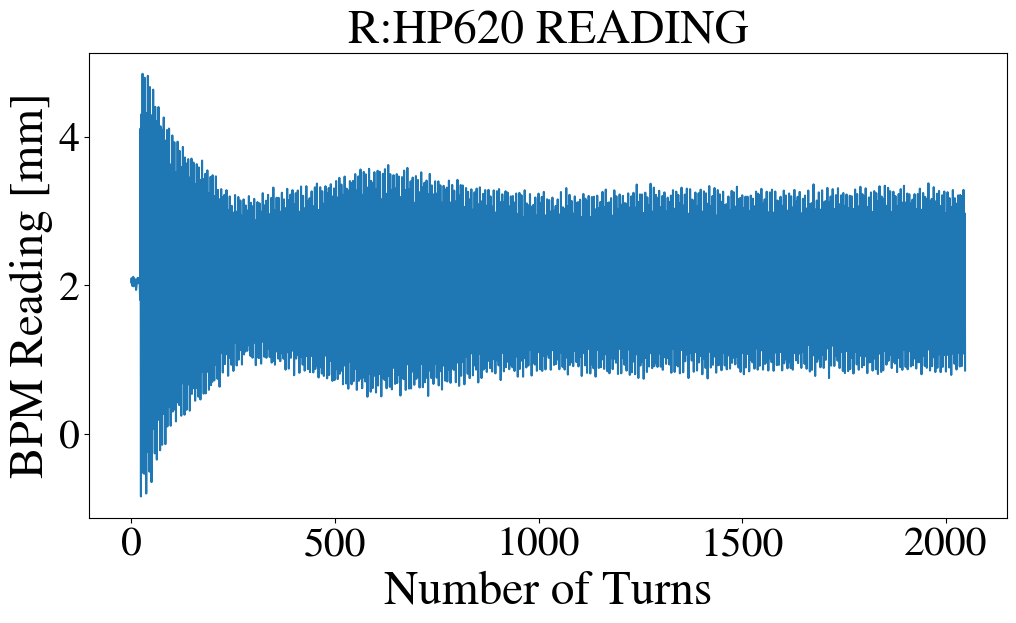
\includegraphics[width=\columnwidth]{chapter3/bpm_kick.png}
   \caption{BPM turn-by-turn data for an arbitrary kick at horizontal BPM R:HP620.}
   \label{fig:bpmkick}
\end{figure}

One important example of using TbT data is using it in order to perform tune measurements. As mentioned in Sec. \ref{sec:basic}, specifically in Eq. \ref{eq:betatron}, the motion inside the Recycler Ring will exhibit betatron oscillations. In particular, the main harmonic of these oscillations will be dictated by the tune frequency. Say a particular set of BPM TbT data has been recorded for $N$ number of turns. Therefore, a Fast-Fourier Transform (FFT) will help uncover and measure to FFT accuracy---$\sigma_Q\approx 1/N $---the main frequency of these oscillations. Figure \ref{fig:bpmfft} shows how the main peak of the FFT can be identified in order to measure the horizontal tune $Q_x$ of the circular accelerator. Furthermore, Ch. \ref{sec:ch4} will explore how a more involved Fourier Transform algorithm, such as NAFF (Numerical Analysis of Fundamental Frequencies) \cite{naff}, will help analyze the spectrum of TbT data and measure higher order harmonics, ultimately, leading to the measurement of RDTs in the RR.     

\begin{figure}[H]
   \centering
   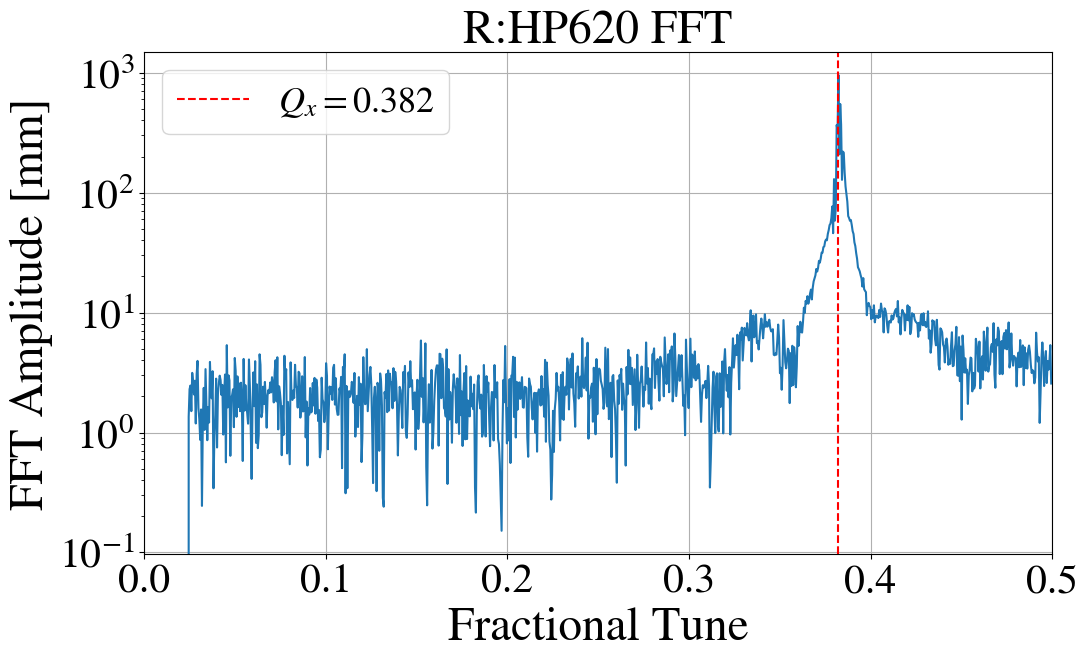
\includegraphics[width=\columnwidth]{chapter3/bpm_fft.png}
   \caption{Fast Fourier Transform amplitude for the turn-by-turn data presented in Fig. \ref{fig:bpmkick}.}
   \label{fig:bpmfft}
\end{figure}

The second type of diagnostics relevant to this work are the Ion Profile Monitors (IPMs). As mentioned before, this device is used to measure the beam size in the Recycler Ring. The RR has two IPM systems: one for the horizontal plane and another one for the vertical. One special characteristic of IPMs relies on their non-destructive nature. The working principle of this system is to collect ions created in the interaction between the proton beam and residual molecules in the vacuum. The secondary ions are detected with micro-channel plates (MCP), which biased at an arbitrary high voltage \cite{betiay}. The counts at each MCP are logged in and digitized in order to be compatible with ACNET. Similar to the BPM systems, an application was developed to control and use the IPM system.     

\begin{figure}[H]
   \centering
   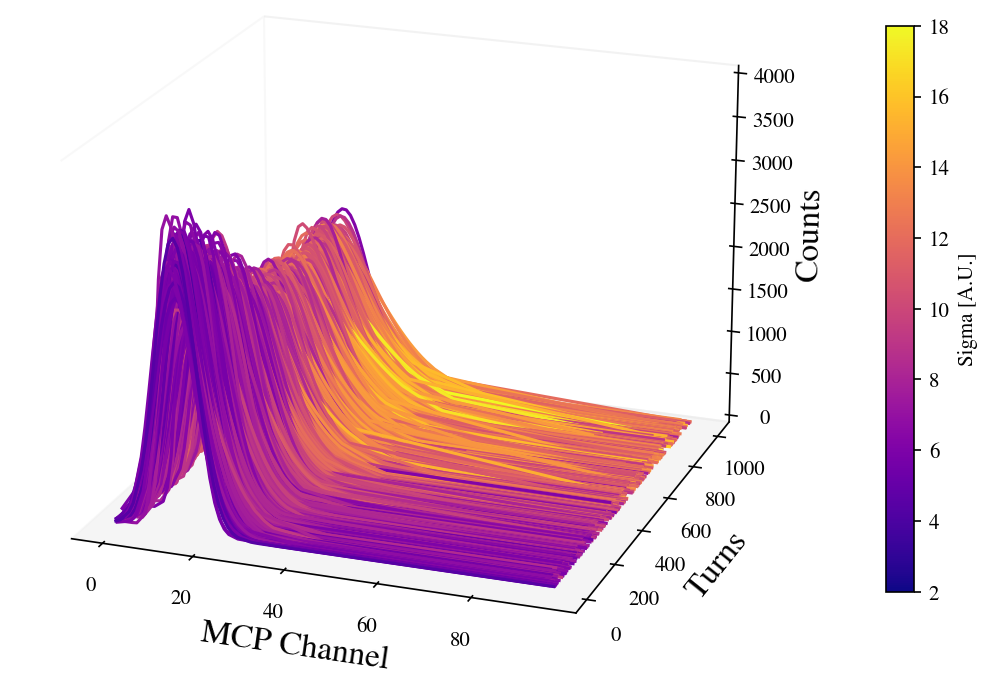
\includegraphics[width=\columnwidth]{chapter3/ipm.png}
   \caption{Reconstructed beam profile for the horizontal plane assuming Gaussian distributions along 1024 turns for an arbitrary beam in the Recycler Ring.}
   \label{fig:ipm0}
\end{figure}

Figure \ref{fig:ipm0} shows the reconstruction of the horizontal beam profile from the raw data of the IPM micro-channel plates. At every turn, the raw count data from each of the 96 MCP is fit to Gaussian beam distribution resulting in some variance $\sigma$. The color map shows the evolution of this beam profile along 1024 turns. The IPM system can record up to 64000 turns. Nevertheless, it batches the data in such a way that it can fit into a $1024 \times 96$ array. In particular, Fig. \ref{fig:ipm0} shows how for this arbitrary experimental conditions, the size of the beam grows with the number of turns---this is pointing at emittance growth. Other distributions different from a Gaussian can be used to fit the raw data in order to extract more information about the skewness or tail population of the beam, e.g., a q-Gaussian or a Skew-Gaussian distribution.

\section{\label{sec:css}Elements for Resonance Compensation}

\begin{figure}[H]
   \centering
   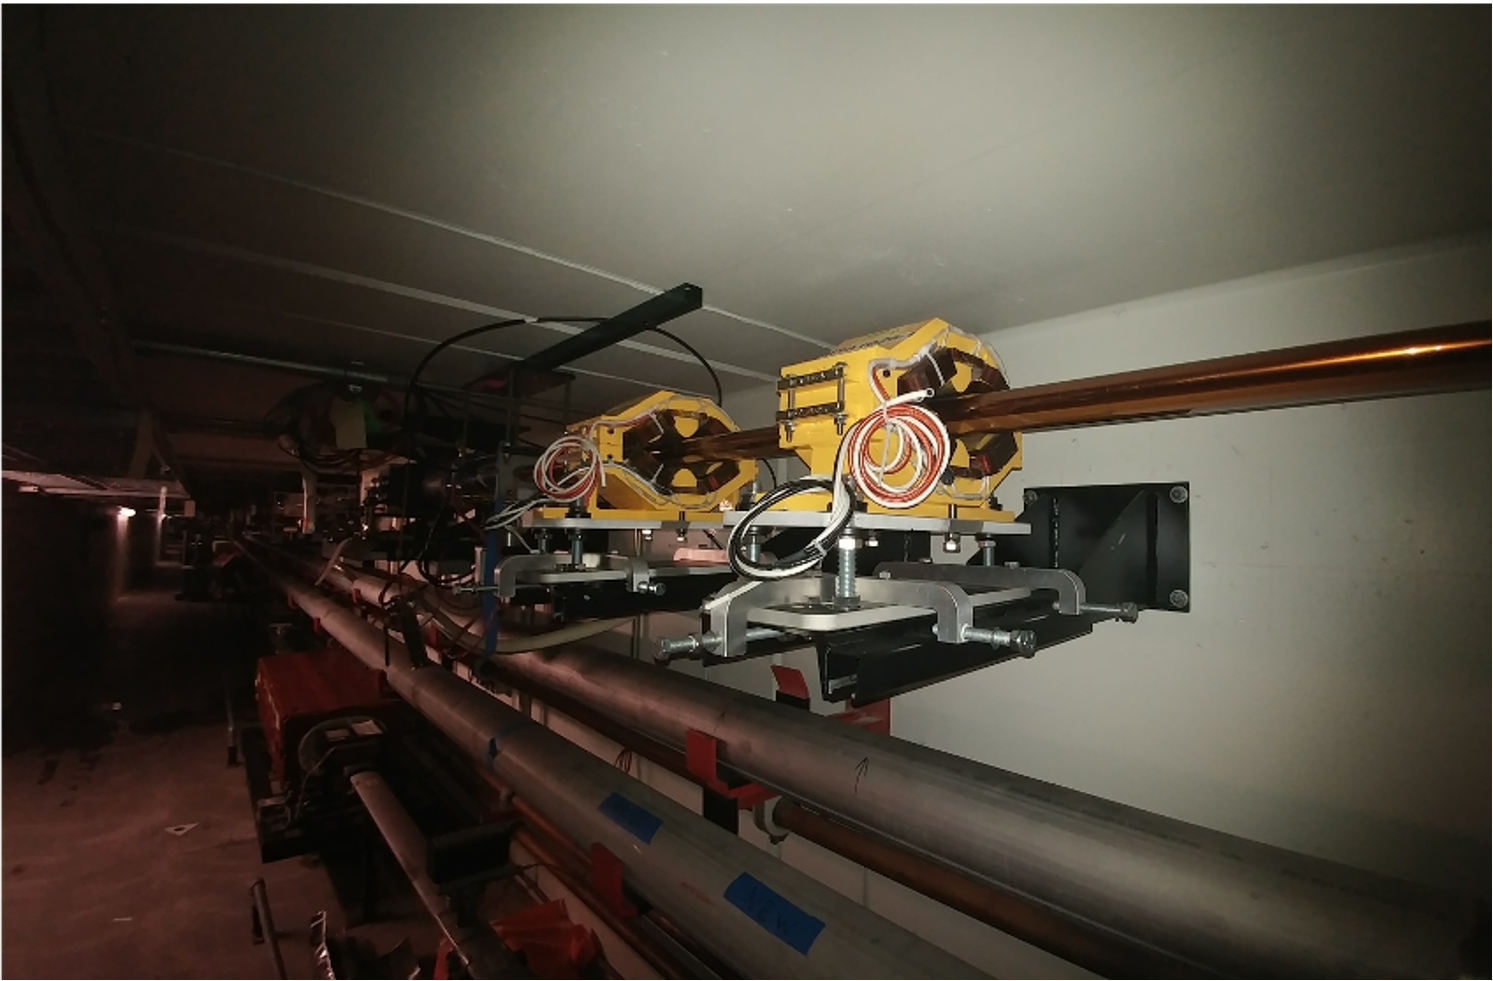
\includegraphics[width=\columnwidth]{chapter3/sextupoles.png}
   \caption{Picture of compensation sextupoles (yellow magnets on top) installed in the Recycler Ring. Picture provided by Dr. Robert Ainsworth.}
   \label{fig:sextupoles}
\end{figure}